%%%%%%%%%%%%%%%%%%%%%%%%%上面的一直到introduction都不用改
\documentclass[sigconf]{acmart}
\settopmatter{authorsperrow=4}
%% \usepackage{adjustbox}
\usepackage{float}
\usepackage{lipsum}

\DeclareMathOperator*{\argmin}{arg\,min}

%% Submission ID.
%% Use this when submitting an article to a sponsored event. You'll
%% receive a unique submission ID from the organizers
%% of the event, and this ID should be used as the parameter to this command.
\acmSubmissionID{pos_xxx}

\citestyle{acmauthoryear}

\AtBeginDocument{%
  \providecommand\BibTeX{{%
    \normalfont B\kern-0.5em{\scshape i\kern-0.25em b}\kern-0.8em\TeX}}}

%\setcopyright{acmcopyright}
%\copyrightyear{2022} 
%\acmYear{2022} 
% \acmDOI{10.1145/3532719.3543260}
%\acmConference{SIGGRAPH '22 Posters}{August 07-11, 2022}{Vancouver, BC, Canada} 
%\acmBooktitle{Special Interest Group on Computer Graphics and Interactive Techniques Conference Posters (SIGGRAPH '22 Posters), August 07-11, 2022}
%\acmDOI{10.1145/3532836.XXXXXX}
%\acmISBN{978-1-4503-9361-4/22/08}


% Figure file shortcut
\newcommand{\putfigure}[1]{\input{fig/#1.tex}}

%%
%% end of the preamble, start of the body of the document source.
\begin{document}

%%
%% The "title" command has an optional parameter,
%% allowing the author to define a "short title" to be used in page headers.
\title{Realistic Compositing of Planar Posters into Live-Action Video}

%%
%% The "author" command and its associated commands are used to define
%% the authors and their affiliations.
%% Of note is the shared affiliation of the first two authors, and the
%% "authornote" and "authornotemark" commands
%% used to denote shared contribution to the research.
\author{Alex Li (Juntao)}
\authornote{Denotes equal contribution.}
\affiliation{%
  \institution{Simon Fraser University}
%  \country{Canada}
}

\author{Zhaoyue Yuan}
\authornotemark[1]
\affiliation{%
  \institution{Simon Fraser University}
%  \country{Canada}
}

\author{Zeyou Peng}
\authornotemark[1]
\affiliation{%
  \institution{Simon Fraser University}
%  \country{Canada}
}

\author{S. Mahdi H. Miangoleh}
\affiliation{%
  \institution{Simon Fraser University}
%  \country{Canada}
}

\author{Ya\u{g}{\i}z Aksoy}
\affiliation{%
  \institution{Simon Fraser University}
%  \country{Canada}
}
%\email{yagiz@sfu.ca}

%%
%% By default, the full list of authors will be used in the page
%% headers. Often, this list is too long, and will overlap
%% other information printed in the page headers. This command allows
%% the author to define a more concise list
%% of authors' names for this purpose.
\renewcommand{\shortauthors}{[Surname1] and [Surname2] et al.}


%% markup


%%
%% The abstract is a short summary of the work to be presented in the
%% article.
%%\begin{abstract}
%%  A clear and well-documented \LaTeX\ document is presented as an
%%  article formatted for publication by ACM in a conference proceedings
%%  or journal publication. Based on the ``acmart'' document class, this
%%  article presents and explains many of the common variations, as well
%%  as many of the formatting elements an author may use in the
%%  preparation of the documentation of their work.
%%\end{abstract}

%%
%% The code below is generated by the tool at http://dl.acm.org/ccs.cfm.
%% Please copy and paste the code instead of the example below.
%%
%%\begin{CCSXML}
%%<ccs2012>
%%   <concept>
%%      <concept_id>10010147.10010371.10010382.10010236</concept_id>
%%       <concept_desc>Computing methodologies~Computational photography</concept_desc>
%%       <concept_significance>500</concept_significance>
%%       </concept>
%% </ccs2012>
%%\end{CCSXML}

%%\ccsdesc[500]{Computing methodologies~Computational photography} % should we change this to something else

%%
%% Keywords. The author(s) should pick words that accurately describe
%% the work being presented. Separate the keywords with commas.
%% parallax scrolling, game development etc.
%%\keywords{texture generation}

%% A "teaser" image appears between the author and affiliation
%% information and the body of the document, and typically spans the
%% page.


%%%%%%%%%%%%%%%%
\begin{teaserfigure}
  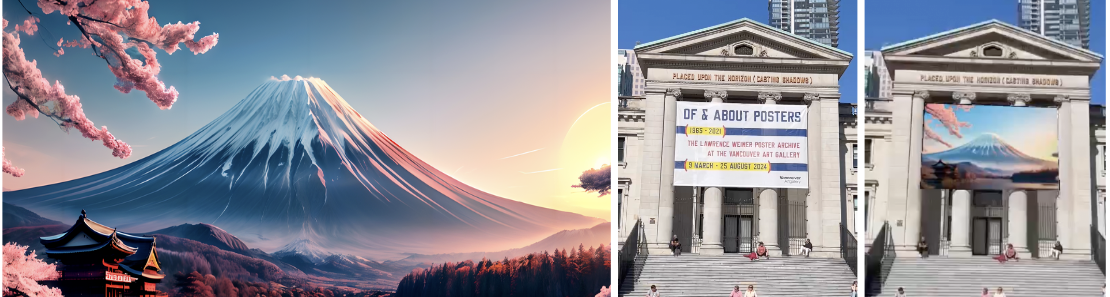
\includegraphics[width=\linewidth]{fig/figure2.png}
  \caption{Input poster, first frame of input video and the first frame of result video}
  \label{fig:teaser}
\end{teaserfigure}

%%
%% This command processes the author and affiliation and ttle
%% information and builds the first part of the formatted document.


%\begin{abstract}
%Abstract
%\end{abstract}

\maketitle

%\placetextbox{0.13}{0.98}{
%
\includegraphics[width=4cm]{cplab.png}
%}
%\placetextbox{0.83}{0.98}{
%Find the project web page here:
%}
%\placetextbox{0.83}{0.965}{
%\textcolor{blue}{\url{http://yaksoy.github.io/parallaxbg/}}
%}



%%%%%%%%%%%%%%%%%%%%%% Part 1 Introduction
\section{Introduction}

The original idea starts with a question: can we replace the poster on the building with our own poster? It leads to several more interesting questions: Will companies try fitting their advertisement on the wall digitally before actually implementing it? What if customers want to see how the poster act in different real-live conditions? So we formulate our project as: Realistic compositing of Planar posters into Live-action Video.

Our project aims to explore and enhance the realm of tracking and compositing by seamlessly integrating planar posters into dynamic live-action sequences. The ultimate goal is to get an output where the input poster maintains a consistent presence, accurately replace and track the designated quadrilateral planar region within the video, and match the changes in perspective, location, and lighting/shading conditions. This realistic compositing strategy can be used in areas such as advertising demos, film production, social media filters or augmented reality, where planar digital contents are coexisting with live-action elements. An example of the input poster and first frame of the input video is shown in figure 1 on the left, and our first frame of the composed output video is on the right.

The whole project can be divided into two parts: tracking and shading. For the tracking portion, our approach includes both the traditional perspective tracking methods and the surface normal-based tracking method, depending on the actual feature in the input video. These methods provides a robust and accurate way to follow the planar region's orientation and position as it moves or changes in the 3D space. 

Shading and lighting play main roles in ensuring that the composited poster's integration appears natural and fusion in the video. We employ shading techniques to match the poster's lighting to the dynamic conditions of the video, preserving the scene's inherent shadows, highlights, and texture nuances, which advertisement or movies have to achieve. Surface normal is estimated by the \textit{Omnidata} model, intrinsic composition, re-scaling, lighting coefficients are applied to the poster and the final albedo harmonization and compositing organize these effects. The result is a fusion of the poster with the input video, where the poster inherits the video's ambient and direct lighting conditions, reacts to environmental changes, and consistently belongs to the space it occupies.



%%%%%%%%%%%%%%%%%%%%%% 
\begin{figure*}[t]
  \centering
  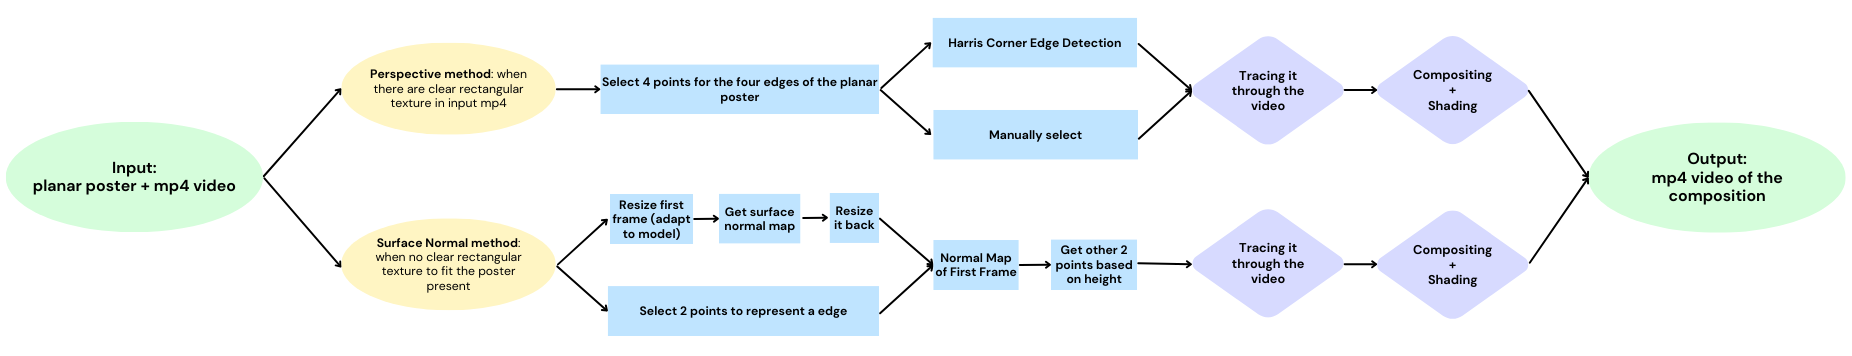
\includegraphics[width=\linewidth]{fig/pipeline.png}
  \caption{Pipeline throughout the project, separated into two cases}
  \label{fig:pipeline}
   \vspace{-0.2cm}
\end{figure*}



%%%%%%%%%%%%%%%%%%%%%% Part 2 Pipeline, method, formulation
\section{pipeline, method, formulation}

The pipeline shown in Figure 2 starts with the input of a poster image and a mp4 video that contains a surface (so that the poster can be stick on). The first step is to identify the type of the video, we divided it into two separate cases. 

The first case is the perspective case, if the planar surface in the video contains a clear quadrilateral region and it stays in the boarder of the video constantly, we can apply the perspective method. The first step is to locate the quadrilateral region in the first frame of the input video. We are selecting the four points manually by clicking the four corners of the quadrilateral, if you do not want to manually select the corners, Harris corner detection is another choice, during the point selecting process, several additional tools are provided such as a magnifier, distance and area calculator, these four points are later used to create a perspective transformation matrix. After this, the next step is to set parameters for the \textit{Lucas-Kanade} optical flow method. Optical flow is used here to track the motion of the selected points between frames. We then enters the main loop which reads each frame of the video in sequence. Each frame is converted to grayscale and \textit{calcOpticalFlowPyrLK} in Cv2 computes the new points of the selected region of the poster based on the changes in different frames. These new points will be tracked and proceeds with the transformation and overlay. Furthermore, when the region is confirmed in the inter-loop of each frame, the poster is warped using perspective transformation matrix M to fit the quadrilateral defined by the corners, plus the OpenCv2 function \textit{warpPerspective}. The mask is then created as the same size as the frame, and a filled polygon is drawn using corner points, the current frame and the warped poster are combined using bitwise operations. By keep updating the to corner points for the next iteration, we get our output video with the poster stays in the quadrilateral region realistically.

The second case is the surface normal case, if the planar surface in the video is "infinite", which a quadrilateral region cannot be select or detected directly, we are using the normal method. The first step involves extracting the first frame from the video and resizing it to a size suitable for the model to process, then the we get the normal map from \textit{Omnidata} such as Figure 3. The normal map is then resized back, to match the resolution of the video frame. We can now select 2 points based on the normal map we get, to define one edge of our quadrilateral region, and input the height of the poster. By evaluating the edge, the height perpendicular to it, and the normal values in this region, we can define the position of the poster in the first frame of the video. After this, we apply similar steps as the perspective method does, for looping and tracking the poster's position by optical flow throughout the video.

In the mean time of looping through the frames for both perspective and normal method, we apply shading. By getting the combined image of the poster and first frame of the video, we apply the following pipeline of methods to this combined image. Firstly, we get the surface normal map from \textit{Omnidata} and use it to determine how light interacts with the surfaces. Then Intrinsic Decomposition is applied to separate the image into its shading (captures the effect of lighting on the scene) and reluctance components. From this, we then get the lighting coefficients which characterize the light's behavior in the scene and use it to ensure that the new shading on the foreground object matches the background lighting. Besides that, albedo harmonization is applied to adjust the composited object's albedo, so that its colors are consistent with the lighting of the scene. The final image is composited by blending the re-shaded poster with the background while respecting the original shading, the normal, and the depth of the scene. With this final image, we can get the shaded poster (based on the shadings of the first frame) and use it as the input poster image throughout the frames loop (since the lighting in the scene of our video is assumed to be not changing).

By combining the points selection, shading and tracing, we get our final output image.


%%%%%%%%%%%%%%%%%%%%%% figure 3
\begin{figure}
  \centering
  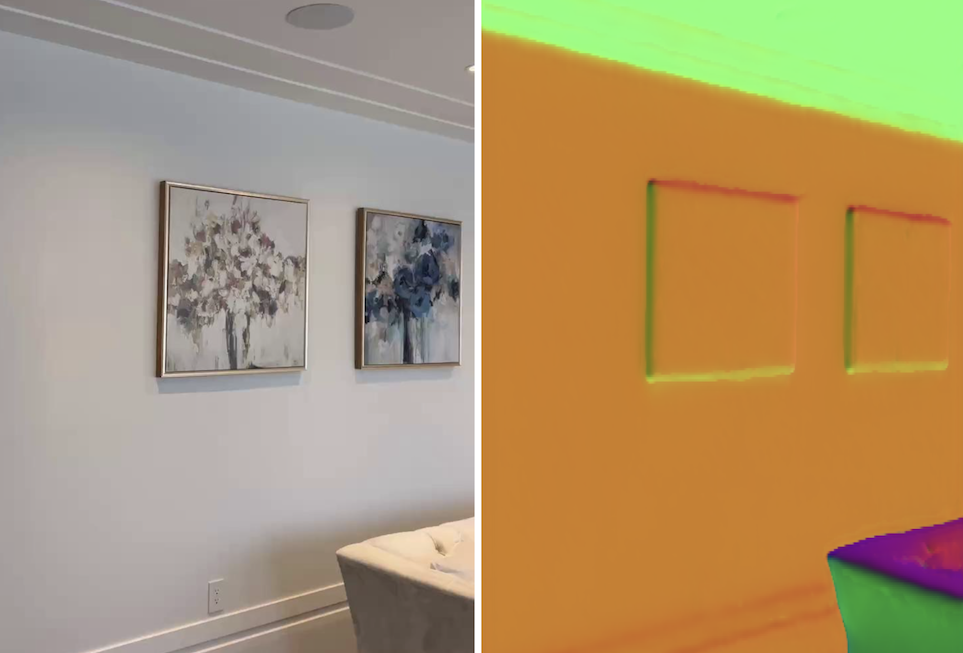
\includegraphics[width=\linewidth]{fig/figure3.png}
  \caption{Example of the normal visualization of the image.}
  \label{fig:texture}
  \vspace{-0.5cm}
\end{figure}
%\putfigure{texture}


%%%%%%%%%%%%%%%%%%%%%% Part 3 results, evaluation, application
\section{Results/Evaluation/Limitation}
\emph{Several results are shown below in Figure 4, since our output is a live-action, we just display the poster, the original first frame and the first frame of the output for comparison and visualization.}

Results for most of our examples are nice and smooth, but it's completeness and perfectness still depend on the input video's texture. For edge cases like the texture of soft materials such as clothes or flags (which might not to be completely planar), or the texture of glasses (might be transparent and show details through it, or consists of complex shadings), it is hard to find a nice normal map for the corner selecting and the tracing process.



%%%%%%%%%%%%%%%%%%%%%% Part 4 Conclusion
\section{Conclusion/Application}

Our project uses advanced tools from computer vision to perfectly blend posters into live-action video scenes. By calculating surface normals or perspective, and tracking movement, we ensure that the poster's position and orientation throughout the video. We also used intrinsic decomposition and other shading tools to adjust the lighting on the poster so it matches the scene perfectly. These techniques help maintain the scene's natural look and improve how the poster fits visually. Our project can be used for advertising, film and movie editing, AR and VR, or further develop for some more straightforward and effective content creation and composition in the future.




%%
%% The acknowledgments section is defined using the "acks" environment
%% (and NOT an unnumbered section). This ensures the proper
%% identification of the section in the article metadata, and the
%% consistent spelling of the heading.
%%\begin{acks}

%%\end{acks}

%%
%% The next two lines define the bibliography style to be used, and
%% the bibliography file.
\bibliographystyle{ACM-Reference-Format}
\bibliography{bibliography}
\cite{bhat2023zoedepth}
\cite{careaga2023intrinsic}
\cite{eftekhar2021omnidata}
\cite{miangoleh2021boosting}
\cite{careaga2023intrinsic2}

\newpage


\begin{figure*}[t]
  \centering
  
\includegraphics[width=\linewidth]{fig/figure4.png}
  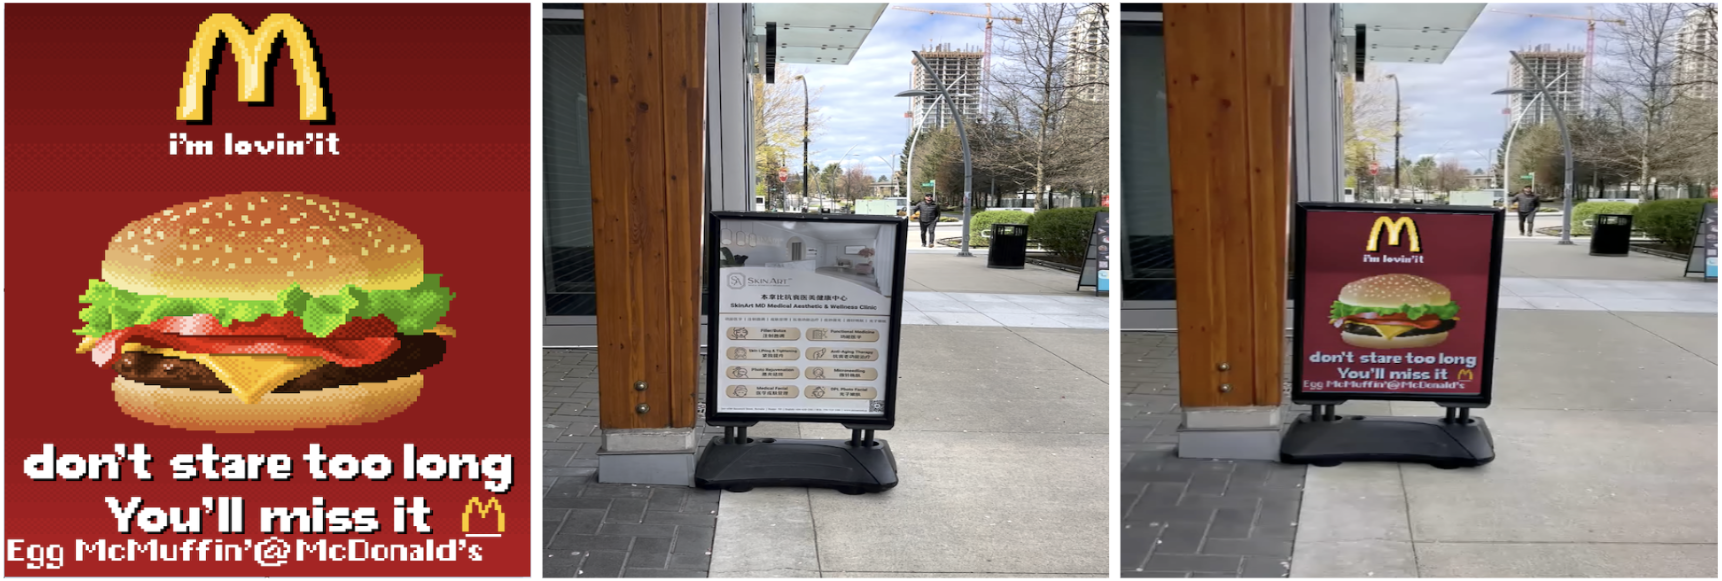
\includegraphics[width=\linewidth]{fig/figure1.png}
  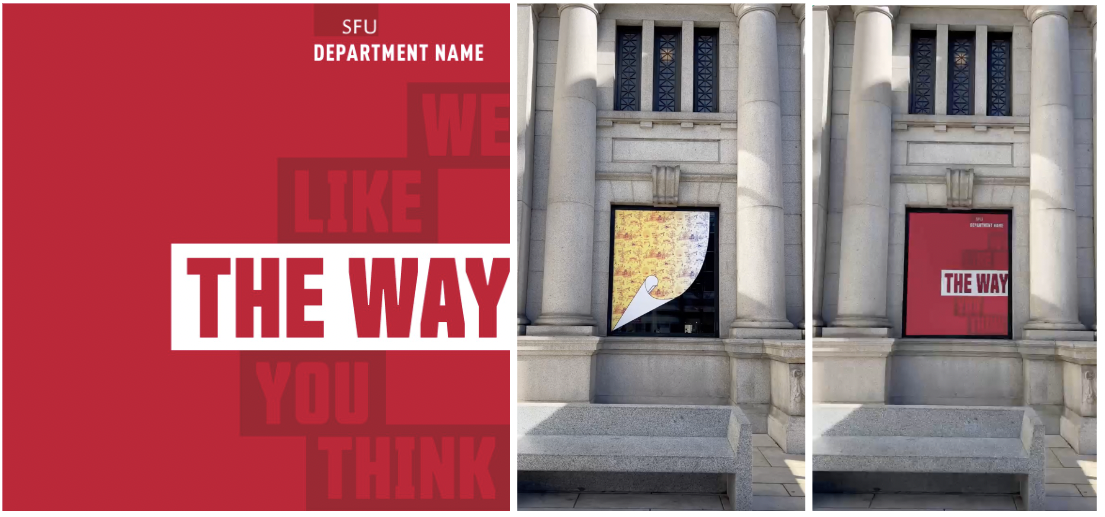
\includegraphics[width=\linewidth]{fig/figure5.png}
  %\caption{Five pairs of our demo visualization, contains the original poster, the first frame of the original video, the first frame of the result video (since video cannot be shown here, check our demo videos}
  \label{fig:pipeline}
   \vspace{-0.2cm}
\end{figure*}

\newpage

\begin{figure*}[t]
  \centering
  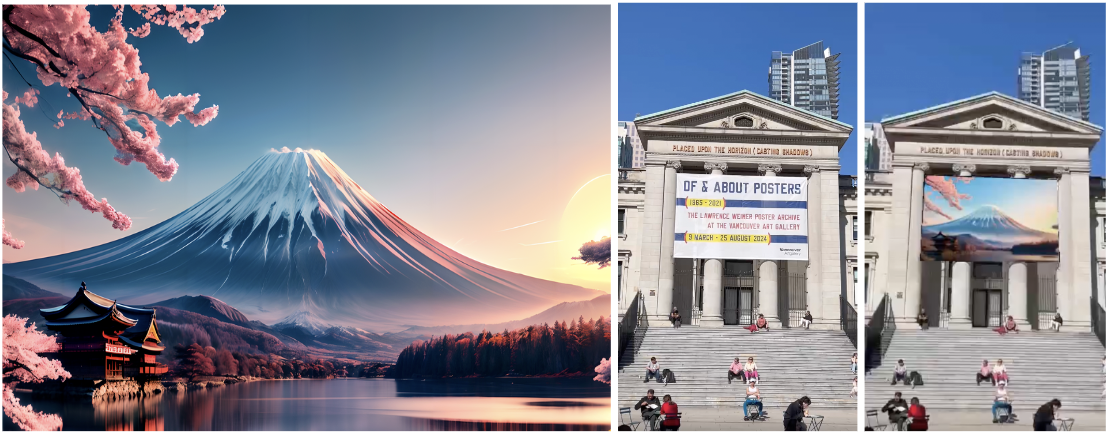
\includegraphics[width=\linewidth]{fig/figure6.png}
  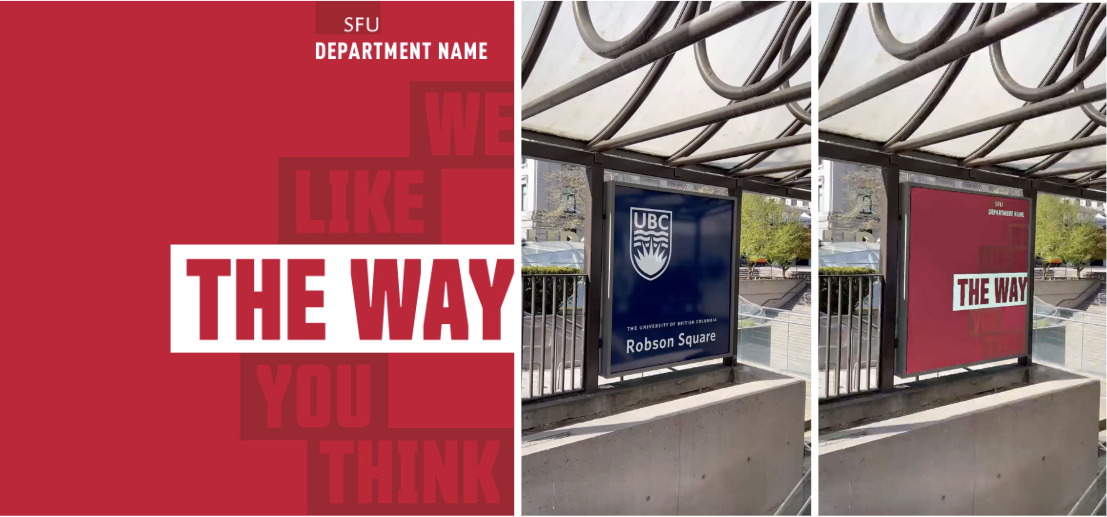
\includegraphics[width=\linewidth]{fig/figure7.png}
  \caption{Five pairs of our demo visualization, contains the original poster, the first frame of the original video, the first frame of the result video (since video cannot be shown here, check our demo videos!)}
  \label{fig:pipeline}
   \vspace{-0.2cm}
\end{figure*}

\end{document}
\endinput
%%
%% End of file `sample-authordraft.tex'.
